%%%%%%%%%%%%%%%%%%%%%%%%%%%%%%%%%%%%%%%%%%%%%%%%%%%%%%%%%%%%%%%%%%%%%%%%%%%%%%%
%                                                                             %
%----------------------------- CONFIGURATION ---------------------------------%
%                                                                             %
%%%%%%%%%%%%%%%%%%%%%%%%%%%%%%%%%%%%%%%%%%%%%%%%%%%%%%%%%%%%%%%%%%%%%%%%%%%%%%%


%------ Document type and options ------%

\documentclass[a4paper,11pt]{article}

%------ Packages ------%

%\usepackage{a4wide}
\usepackage{amsmath}
\usepackage{amssymb}
\usepackage{array} %%custom arrays
\usepackage[french]{babel}
\usepackage{bm} %%bold characters in math mode
\usepackage[makeroom]{cancel} %%to cancel (bar) a term in an equation
\usepackage[justification=centering, textfont={small}, labelfont={bf}]{caption}
\usepackage{color} %%fancy colours
\usepackage{dsfont}
\usepackage{enumitem} %%custom enumeration elements
\usepackage{empheq} %eqnarray with left brace
%\usepackage{fancybox}
%\usepackage{fancyhdr}
\usepackage[T1]{fontenc}
%\usepackage{framed}
\usepackage{fullpage}
\usepackage[top=2cm, bottom=2cm, left=2cm, right=2cm]{geometry}
\usepackage{graphicx}
%\usepackage{hangcaption}
\usepackage[hidelinks]{hyperref} %hyper links, hidden
\usepackage{indentfirst}
\usepackage[utf8]{inputenc}
%\usepackage{lastpage}
\usepackage{listings}
%\usepackage{makecell} %CR in tabular cell
\usepackage{mathtools} %boxes in align environment
%\usepackage{moreverb}
\usepackage{multirow}% multirows in table
\usepackage{sectsty}
\usepackage[squaren,Gray]{SIunits} %%writing physics, compatible with amssymb and pstricks
\usepackage{stmaryrd} %%double brackets
%\usepackage{subcaption}
%\usepackage{textcomp} %%for TM (\texttrademark)and other symbols
\usepackage[x11names]{xcolor}
\usepackage{titlesec} %%custom section titles
\usepackage[nottoc]{tocbibind} % table of contents
\usepackage{url}
\usepackage{xspace}

% Matrix style
\usepackage{tikz}
\usetikzlibrary{matrix, positioning, fit}

% Tensor notation
\usepackage{stackengine}
\newcommand\barbelow[1]{\stackunder[1.2pt]{$#1$}{\rule{.8ex}{.075ex}}}

%------ Parameters ------%

\setlength\parindent{24pt}

% Caption parameters, for figures, subfigures
%\captionsetup[figure]{format=hang, labelsep=colon, font=small, labelfont=bf}
%\captionsetup[subfigure]{format=plain, labelformat=parens, labelsep=space,
%                         font=footnotesize, labelfont=up}

% Practical shortcuts for math writing:
\newcommand{\dx}{\,dx}
\newcommand{\ito}{,\dotsc,}
\newcommand{\R}{\mathbb{R}}
\newcommand{\N}{\mathbb{N}}
\newcommand{\Z}{\mathbb{Z}}
\newcommand{\Poly}[1]{\mathcal{P}_{#1}}
\newcommand{\abs}[1]{\left\lvert#1\right\rvert}
\newcommand{\norm}[1]{\left\lVert#1\right\rVert}
\newcommand{\pars}[1]{\left(#1\right)}
\newcommand{\bigpars}[1]{\bigl(#1\bigr)}
\newcommand{\set}[1]{\left\{#1\right\}}
\newcommand{\dsp}{\displaystyle}
\DeclareMathOperator{\Tr}{Tr}

% Large number of matrix columns
\setcounter{MaxMatrixCols}{12}

% bold letters for vectors
\newcommand{\bd}{\mathbf{d}}

\newcommand{\bD}{\mathbf{D}}
\newcommand{\bM}{\mathbf{M}}
\newcommand{\bN}{\mathbf{N}}
\newcommand{\bQ}{\mathbf{Q}}
\newcommand{\bS}{\mathbf{S}}

\newcommand{\beps}{\bm{\epsilon}}
\newcommand{\bsig}{\bm{\sigma}}
\newcommand{\Be}{\mathbf{B_e}}
\newcommand{\dif}{\mathrm{d}}

% Tensor notation
\newcommand{\stens}{\barbelow{\barbelow{s}}}
\newcommand{\sigtens}{\barbelow{\barbelow{\sigma}}}
\newcommand{\Itens}{\barbelow{\barbelow{I}}}
\newcommand{\Stens}{\barbelow{\barbelow{\barbelow{S}}}}
\newcommand{\Ttens}{\barbelow{\barbelow{\barbelow{T}}}}

% Practical shortcuts for math writing:
%with package SIunits
\newcommand{\cm}{\centi\meter}
\newcommand{\mm}{\milli\meter}
\newcommand{\microm}{\micro\meter}
% Font shortcuts
\newcommand{\gr}{\textbf}
\newcommand{\un}{\underline}
\newcommand{\se}{\textsf}
\newcommand{\te}{\texttt}
\newcommand{\al}{\textit{et al}. }
\newcommand{\ie}{\textit{i}.\textit{e}. }

% Reference aliases
\newcommand{\figref}[1]{\hyperref[#1]{\te{Figure \ref{#1}}}}
\newcommand{\algoref}[1]{\hyperref[#1]{\te{Algorithme \ref{#1}}}}
\newcommand{\secref}[1]{\hyperref[#1]{section \ref{#1}}}
\newcommand{\chapref}[1]{\hyperref[#1]{chapitre \ref{#1}}}
\newcommand{\tabref}[1]{\hyperref[#1]{\te{table \ref{#1}}}}
\newcommand{\annexeref}[1]{\hyperref[#1]{annexe \ref{#1}}}

% Title colours
\xdefinecolor{color1}{named}{DeepSkyBlue4}
\xdefinecolor{color2}{named}{DeepSkyBlue3}
\xdefinecolor{color3}{named}{DeepSkyBlue1}
\sectionfont{\color{color1}}
\subsectionfont{\color{color1}}
\subsubsectionfont{\color{color1}}

% Title indent, /!\ with package "titlesec"
% %\titlespacing{command}{left spacing}{before spacing}{after spacing}[right]
% \titlespacing{\section}{0ex}{1ex}{3ex}{}
% \titlespacing{\subsection}{5ex}{2ex}{2ex}{}
% \titlespacing{\subsubsection}{10ex}{0}{0}{}




%%%%%%%%%%%%%%%%%%%%%%%%%%%%%%%%%%%%%%%%%%%%%%%%%%%%%%%%%%%%%%%%%%%%%%%%%%%%%%%
%                                                                             %
%------------------------------- BODY ----------------------------------------%
%                                                                             %
%%%%%%%%%%%%%%%%%%%%%%%%%%%%%%%%%%%%%%%%%%%%%%%%%%%%%%%%%%%%%%%%%%%%%%%%%%%%%%%

% titre, auteur et date
\title{}
\author{Camille Krewcun \\ \scriptsize{Inria - DEFROST} }
\date{\today}

\begin{document}
\maketitle

Derivation of the shape functions representing a Timoshenko beam element with 12
Degrees of Freedom (DoF), with a local frame located in the middle of the beam, as
represented on \figref{beam_local_middle_frame}. We follow the same computation
steps as in \cite{Baz03}, in which the local frame is considered at node $N_1$.

\begin{figure}[!h]
	\centering
	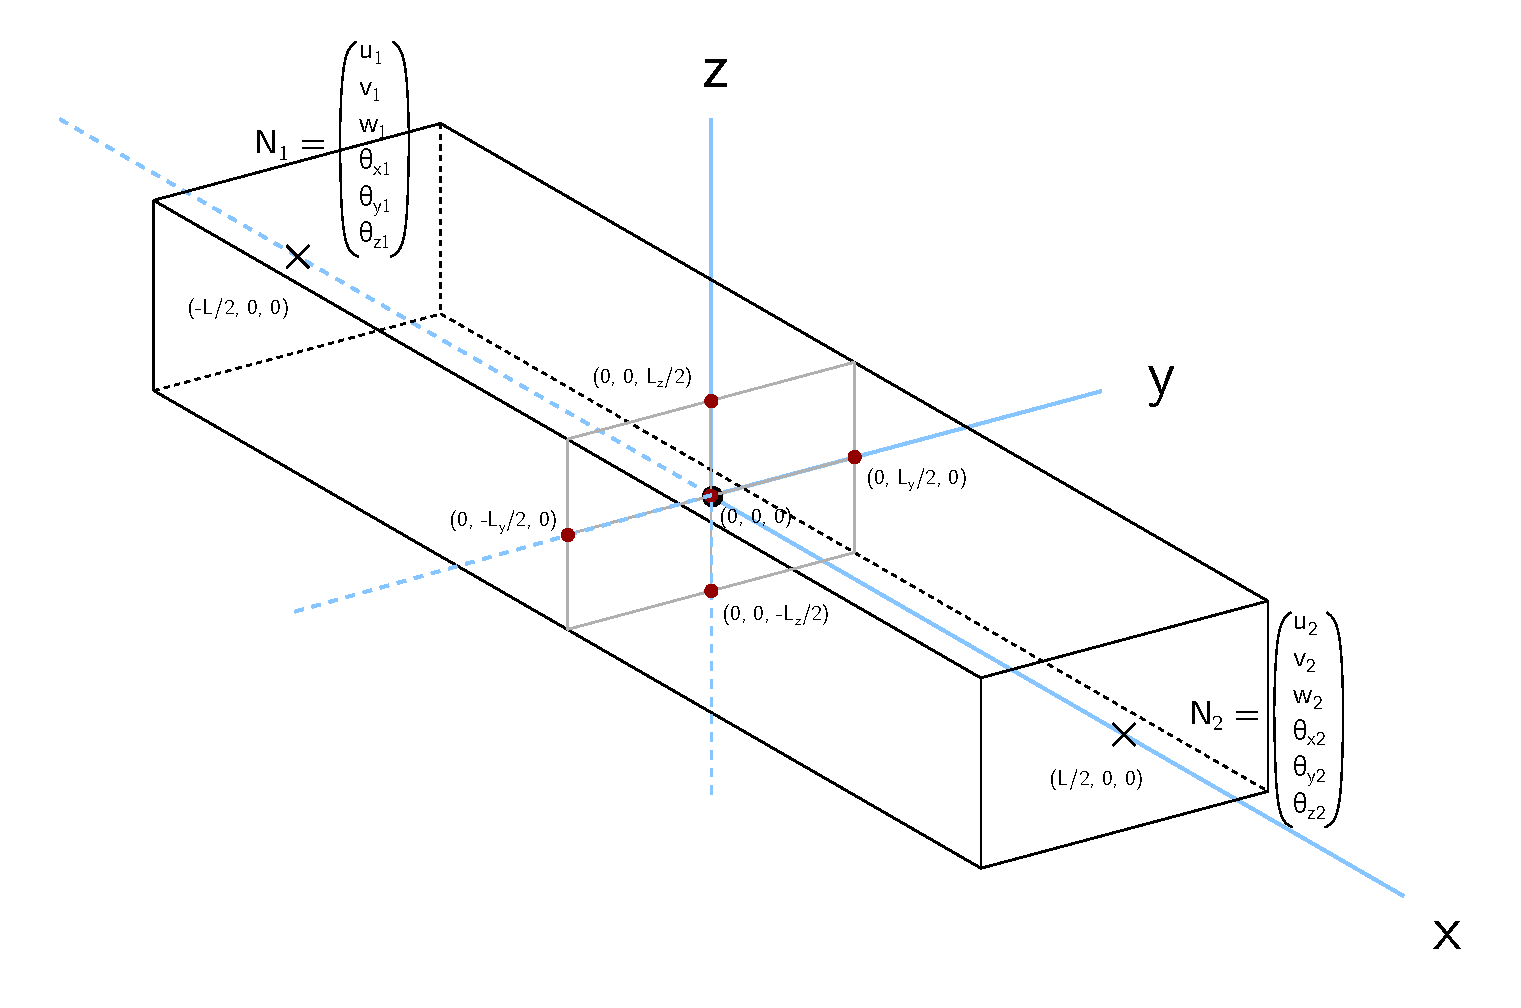
\includegraphics[scale=0.35]{Images/beam_local_middle_frame}
	\caption{Beam element, defined by two 6 DoFs nodes $N_1$ and $N_2$, with a
local frame located at the centre of the beam. Length: $L$, section dimensions:
$L_y$, $L_z$.}
	\label{beam_local_middle_frame}
\end{figure}

\section*{Timoshenko beam shape functions - middle frame}

\subsection*{Base hypotheses}

As in \cite{Baz03}, we aim at expressing a continuous displacement field $\bd \in
\R^3$ in the beam element, as a function of the discrete node's displacement $\bD
\in \R^{12}$ defined as :
\begin{equation}
\bD =
\begin{pmatrix}
	u_1 & v_1 & w_1 & \theta_{x1} & \theta_{y1} & \theta_{z1} &
	u_2 & v_2 & w_2 & \theta_{x2} & \theta_{y2} & \theta_{z2}
\end{pmatrix}^T,
\end{equation}
where $\{u_i, v_i, w_i\}$ represent translation of node $i$ along the $x$, $y$, and
$z$ axes respectively, and $\{\theta_{xi}, \theta_{yi}, \theta_{zi}\}$ its rotation
around each axis.\\

We want to find $\bN \in \R^{3\times12}$ such that:
\begin{equation} \label{eq:d_expr}
	\bd(x,y,z) = \bN(x,y,z)\bD.
\end{equation}

\cite{Baz03}: kinematic relations for a 3D beam undergoing axial, torsional, and
bending deformations in the (xy)- and (xz)-planes
\begin{equation} \label{eq:displacement}
\left\{
	\begin{aligned}
		d_x & = u - y \left(\frac{\partial v}{\partial x}\right) - z \left(\frac{\partial w}{\partial x}\right) \\
		d_y & = -z\theta_x + v \\
		d_z & = y\theta_x + w,
	\end{aligned}
\right.
\end{equation}
where:
\begin{itemize}[label=$\gr{-}$, font=\LARGE, font=\color{black}, topsep = 0.2cm,
itemsep=0.2cm]
	\item $\bd = (d_x, d_y, d_z)^T$,
	\item translations $(v, w)$ consist of contributions $(v_b, w_b)$ and $(v_s,
w_s)$ due respectively to bending and transverse shear.\\
\end{itemize}

Relationships between total slope (?), bending rotation and transverse shear are:
\begin{align}
\frac{\partial v}{\partial x} & = \frac{\partial v_b}{\partial x} + \frac{\partial v_s}{\partial x} = \theta_z + \gamma_{xy}, \label{eq:dv_dx}\\
\frac{\partial w}{\partial x} & = \frac{\partial w_b}{\partial x} + \frac{\partial w_s}{\partial x} = -\theta_y + \gamma_{xz}, \label{eq:dw_dx}
\end{align}
where $\gamma_{xy}$ and $\gamma_{xz}$ are shear strains in the $(xy)$- and $(xz)$-
planes, respectively.\\
Relation between the rotations $(\theta_y, \theta_z)$ and the bending deformations
$(v_b, w_b)$:
\begin{align}
\theta_z & = \frac{\partial v_b}{\partial x}, \label{eq:theta_z_dv_dx} \\
\theta_y & = - \frac{\partial w_b}{\partial x}. \label{eq:theta_y_dw_dx}
\end{align}
\underline{NB}: Axial warping displacement during torsion is ignored.

\subsection*{Computation of shape functions}

\subsubsection*{Axial and torsional deformation}

Linear shape functions, included for completeness. Classic shape function matrices
for axial and torsional deformation :
\begin{equation}
	[ \mathcal{N}_u(\xi)] = \begin{pmatrix} 1-\xi & \xi \end{pmatrix},
\end{equation}
\begin{equation}
	[\mathcal{N}_{\theta_x}(\xi)] = \begin{pmatrix} 1-\xi & \xi \end{pmatrix},
\end{equation}
where $\xi = \frac{x}{l}$ (dimensionless axial coordinate). Which can be
alternatively written:
\begin{equation} \label{eq:u_expr}
	u = \begin{pmatrix} 1-\xi & \xi \end{pmatrix} \begin{pmatrix} u_1 \\ u_2 \end{pmatrix} = (1-\xi)u_1 + \xi u_2,
\end{equation}
and
\begin{equation} \label{eq:theta_x_expr}
	\theta_x = \begin{pmatrix} 1-\xi & \xi \end{pmatrix} \begin{pmatrix} \theta_{x1} \\ \theta_{x2} \end{pmatrix} = (1-\xi)\theta_{x1} + \xi \theta_{x2}.
\end{equation}


\subsubsection*{bending deformation in the (xy)-plane}

/!$\backslash$ Contrarily to axial and torsional deformation, shape functions used
for translational and rotational bending deformations are the conventional
\textbf{cubic} Hermitian polynomials => continuity and completeness conditions +
shear deformation parameters (accounting for the effect of shear).\\

\noindent \underline{Assumptions} \cite{Nar74}:\\
$\bullet$ The translation deformation $v(x)$ at an arbitrary location $x$ is
expressed as
\begin{equation} \label{eq:v_expr}
	v(x) = a_0 + a_1x + a_2x^2 + a_3x^3,
\end{equation}
where the $a_i \in \R$ are coefficients depending on the nodes DoFs.\\
$\bullet$ The shear strain is independent of $x$, \ie constant along the element
\begin{equation} \label{eq:gamma_0}
	\gamma_{xy} = const = \gamma_0.\\
\end{equation}

\noindent The relation between the bending moment $\bM_z$ and the shear force
$\bQ_y$ is
\begin{equation} \label{eq:relation_M_z_Q_y}
	\frac{\dif \bM_z}{\dif x} - \bQ_y = 0,
\end{equation}
and the moment-curvature relationship is
\begin{equation} \label{eq:M_z}
	\bM_z = -EI_{zz}\frac{\partial \theta_z}{\partial x},
\end{equation}
where $I_{zz}$ is the section second moment of area about the z-axis.\\
The shear force is also related to the transverse shear strain by
\begin{equation}
	\bQ_y = \kappa_yGA\gamma_{xy},
\end{equation}
where $\kappa_y$ is the shear correction factor that accounts for the non-uniform
distribution of the shear stress over the cross-section of area $A$, $E$ is the
Young's modulus, and $G$ the shear modulus such that
\begin{equation}
	G = \frac{E}{2(1+\nu)}.\\
\end{equation}

\noindent From \eqref{eq:dv_dx}, \eqref{eq:v_expr} and \eqref{eq:gamma_0} we have:
\begin{align}
	\frac{\partial v}{\partial x} = \theta_z + \gamma_{xy} & \implies a_1 + 2a_2x + 3a_3x^2 = \theta_z + \gamma_0 \label{eq:theta_z_int} \\
	& \implies \frac{\partial \theta_z}{\partial x} = 2a_2 + 6a_3x. \label{eq:theta_z_int_2}
\end{align}
From \eqref{eq:M_z} we then have
\begin{equation}
	\bM_z = -EI_{zz}\frac{\partial \theta_z}{\partial x} = -EI_{zz}(2a_2 + 6a_3x)
\end{equation}
and
\begin{equation}
	\frac{\dif \bM_z}{\dif x} = -6EI_{zz}a_3.
\end{equation}
Replacing $\bM_z$ and $\bQ_y$ by their expressions in \eqref{eq:relation_M_z_Q_y}
gives:
\begin{align}
\kappa_y G A \gamma_0 & = -6EI_{zz}a_3 \\
\gamma_0 & = -6\Lambda_z a_3,
\end{align}
where we define $\Lambda_z$ as:
\begin{equation}
	\Lambda_z = \frac{EI_{zz}}{\kappa_y G A}.
\end{equation}
Replacing $\gamma_0$ by this expression in \eqref{eq:theta_z_int}, we obtain
\begin{equation} \label{eq:theta_z}
	\theta_z = a_1 + 2a_2x + (3x^2 + 6\Lambda_z)a_3.\\
\end{equation}

\noindent Next, the expressions of the $\{a_i\}$ coefficients are obtained
satisfying the beam's boundary conditions. /!$\backslash$ Here the computation
differs from \cite{Baz03}, as we do not consider the same local frame.
Therefore, the boundary conditions associted with a middle local frame are :
\begin{align}
v\left(-\frac{l}{2}\right) & = v_1 \text{\hspace{20mm}} \theta_z \left(-\frac{l}{2}\right) = \theta_{z1}, \label{eq:BC_node_1} \\
v\left(\frac{l}{2}\right) & = v_2 \text{\hspace{23mm}} \theta_z \left(\frac{l}{2}\right) = \theta_{z2}. \label{eq:BC_node_2}
\end{align}
From \eqref{eq:BC_node_1} and \eqref{eq:BC_node_2}, we can derive the following
computation:
\begin{align}
v_2 + v_1 & = v\left(-\frac{l}{2}\right) + v\left(\frac{l}{2}\right), \nonumber \\
	& = a_0 - \frac{l}{2}a_1 + \frac{l^2}{4}a_2 - \frac{l^3}{8}a_3 + a_0 + \frac{l}{2}a_1 + \frac{l^2}{4}a_2 + \frac{l^3}{8}a_3, \nonumber \\
v_1 + v_2 & = 2a_0 + \frac{l^2}{2}a_2, \label{eq:BC1}
\end{align}
\begin{align}
v_2 - v_1 & = v\left(\frac{l}{2}\right) - v\left(-\frac{l}{2}\right), \nonumber \\
	& = a_0 + \frac{l}{2}a_1 + \frac{l^2}{4}a_2 + \frac{l^3}{8}a_3 - a_0 + \frac{l}{2}a_1 - \frac{l^2}{4}a_2 + \frac{l^3}{8}a_3, \nonumber \\
v_2 - v_1 & = la_1 + \frac{l^3}{4}a_3, \label{eq:BC2}
\end{align}
\begin{align}
\theta_{z2} + \theta_{z1} & = \theta_z \left(\frac{l}{2}\right) + \theta_z \left(-\frac{l}{2}\right), \nonumber \\
	& = a_1 + la_2 + \left( \frac{3l^2}{4} + 6\Lambda_z \right)a_3 + a_1 - la_2 + \left( \frac{3l^2}{4} + 6\Lambda_z \right)a_3, \nonumber \\
\theta_{z2} + \theta_{z1} & = 2a_1 + \left( \frac{3l^2}{2} + 12\Lambda_z \right)a_3, \label{eq:BC3}
\end{align}
\begin{align}
\theta_{z2} - \theta_{z1} & = \theta_z \left(\frac{l}{2}\right) - \theta_z \left(-\frac{l}{2}\right), \nonumber \\
	& = a_1 + la_2 + \left( \frac{3l^2}{4} + 6\Lambda_z \right)a_3 - a_1 + la_2 - \left( \frac{3l^2}{4} + 6\Lambda_z \right)a_3, \nonumber \\
\theta_{z2} - \theta_{z1} & = 2la_2. \label{eq:BC4}
\end{align}

\noindent From \eqref{eq:BC4}, we have directly
\begin{equation}
	a_2 = \frac{\theta_{z2} - \theta_{z1}}{2l}.
\end{equation}
Replacing $a_2$ in \eqref{eq:BC1}, we obtain
\begin{align}
v_1 + v_2 & = 2a_0 + \frac{l^2(\theta_{z2} - \theta_{z1})}{4l}, \nonumber \\
a_0 & = \frac{1}{2} \left( v_1 + v_2 - \frac{l(\theta_{z2} - \theta_{z1})}{4} \right).
\end{align}
Then we can solve \eqref{eq:BC2} and \eqref{eq:BC3} for $a_1$ and $a_3$ :

\begin{empheq}[left={\empheqlbrace}]{alignat=1}
    v_2 - v_1 & = la_1 + \frac{l^3}{4}a_3 \label{eq:a_1_a_3_1}\\
    \theta_{z2} + \theta_{z1} & = 2a_1 + \left( \frac{3l^2}{2} + 12\Lambda_z \right)a_3 .\label{eq:a_1_a_3_2}
\end{empheq}
Equation \eqref{eq:a_1_a_3_1} gives
\begin{equation} \label{eq:a_1_int}
	a_1 = \frac{v_2 - v_1}{l} - \frac{l^2}{4}a_3,
\end{equation}
which can be replaced into \eqref{eq:a_1_a_3_2}:
\begin{align}
\theta_{z2} + \theta_{z1} & = 2 \left( \frac{v_2 - v_1}{l} - \frac{l^2}{4}a_3 \right) + \left( \frac{3l^2}{2} + 12\Lambda_z \right)a_3, \nonumber\\
\theta_{z2} + \theta_{z1} & = \frac{2}{l}(v_2-v_1) - \frac{l^2}{2}a_3 + \left( \frac{3l^2}{2} +12\Lambda_z \right)a_3, \nonumber\\
\theta_{z2} + \theta_{z1} -\frac{2}{l}(v_2-v_1) & = (l^2 + 12\Lambda_z)a_3, \nonumber\\
a_3 & = \frac{1}{l^2 + 12\Lambda_z} \left[ \theta_{z2} + \theta_{z1} -\frac{2}{l}(v_2-v_1) \right]. \nonumber
\end{align}
Defining $\Phi_z$ (the shear deformation parameter which represents the ratio
between bending and shear stiffnesses) as
\begin{equation}
	\Phi_z = \frac{12\Lambda_z}{l^2},
\end{equation}
and $\bar{\Phi_z}$ as
\begin{equation}
	\bar{\Phi}_z = \frac{1}{1 + \Phi_z},
\end{equation}
we have the following expression of $a_3$:
\begin{equation}
a_3 = \frac{\bar{\Phi}_z}{l^2} \left( \theta_{z2} + \theta_{z1} -\frac{2}{l}(v_2-v_1) \right).
\end{equation}
Finally, going back to \eqref{eq:a_1_int} we obtain
\begin{equation}
a_1 = \frac{v_2 - v_1}{l} - \frac{\bar{\Phi}_z}{4} \left[ \theta_{z2} + \theta_{z1} -\frac{2}{l}(v_2-v_1) \right]
\end{equation}
Summarizing:
\begin{equation}
\left\{
	\begin{aligned}
		a_0 & = \frac{1}{2} \left( v_1 + v_2 - \frac{l(\theta_{z2} - \theta_{z1})}{4} \right), \\
		a_1 & = \frac{v_2 - v_1}{l} - \frac{\bar{\Phi}_z}{4} \left[ \theta_{z2} + \theta_{z1} -\frac{2}{l}(v_2-v_1) \right], \\
		a_2 & = \frac{\theta_{z2} - \theta_{z1}}{2l}, \\
		a_3 & = \frac{\bar{\Phi}_z}{l^2} \left( \theta_{z2} + \theta_{z1} -\frac{2}{l}(v_2-v_1) \right).
	\end{aligned}
\right.
\end{equation}

\noindent Substituting the $a_i$ by their expressions in \eqref{eq:v_expr}, we get
\begin{align*}
v(x) & = \frac{1}{2} \left( v_1 + v_2 - \frac{l(\theta_{z2} - \theta_{z1})}{4} \right) + \left[ \frac{v_2 - v_1}{l} - \frac{\bar{\Phi}_z}{4} \left( \theta_{z2} + \theta_{z1} -\frac{2}{l}(v_2-v_1) \right) \right] x \\
	& \text{\hspace{4mm}} + \frac{\theta_{z2} - \theta_{z1}}{2l} x^2 + \frac{\bar{\Phi}_z}{l^2} \left( \theta_{z2} + \theta_{z1} -\frac{2}{l}(v_2-v_1) \right) x^3 \\
v(x) & = \left[ \frac{1}{2} - \left( \frac{1}{l} + \frac{\bar{\Phi}_z}{2l} \right) x + \frac{2\bar{\Phi}_z}{l^3}x^3 \right]v_1 + \left( \frac{l}{8} - \frac{\bar{\Phi}_z}{4}x - \frac{1}{2l}x^2 + \frac{\bar{\Phi}_z}{l^2}x^3 \right)\theta_{z1} \\
	& \text{\hspace{4mm}} + \left[ \frac{1}{2} + \left( \frac{1}{l} + \frac{\bar{\Phi}_z}{2l}\right)x - \frac{2\bar{\Phi}_z}{l^3}x^3 \right]v_2 + \left( -\frac{l}{8} - \frac{\bar{\Phi}_z}{4}x + \frac{1}{2l}x^2 + \frac{\bar{\Phi}_z}{l^2}x^3 \right)\theta_{z2}.
\end{align*}
Replacing $x$ by $\xi = \frac{x}{l}$, we have:
\begin{align}
	v(\xi) & = \left( \frac{1}{2} - \frac{2 + \bar{\Phi}_z}{2}\xi + 2\bar{\Phi}_z\xi^3 \right)v_1 + \left( \frac{l}{8} - \frac{l\bar{\Phi}_z}{4}\xi - \frac{l}{2}\xi^2 + l\bar{\Phi}_z\xi^3 \right)\theta_{z1} \nonumber\\
		& \text{\hspace{4mm}} + \left( \frac{1}{2} + \frac{2 + \bar{\Phi}_z}{2}\xi - 2\bar{\Phi}_z\xi^3 \right)v_2 + \left( -\frac{l}{8} - \frac{l\bar{\Phi}_z}{4}\xi + \frac{l}{2}\xi^2 + l\bar{\Phi}_z\xi^3 \right)\theta_{z2} \nonumber\\
	v(\xi) & = \frac{1}{2} \left[1 - (2 + \bar{\Phi}_z)\xi + 4\bar{\Phi}_z\xi^3 \right] v_1 + \frac{l}{8}\left(1 - 2\bar{\Phi}_z\xi - 4\xi^2 + 8\bar{\Phi}_z\xi^3 \right) \theta_{z1} \nonumber\\
		& \text{\hspace{4mm}} + \frac{1}{2} \left[1 + (2 + \bar{\Phi}_z)\xi - 4\bar{\Phi}_z\xi^3 \right] v_2 + \frac{l}{8}\left( -1 - 2\bar{\Phi}_z\xi + 4\xi^2 + 8\bar{\Phi}_z\xi^3 \right) \theta_{z2}.
\end{align}
Hence, $v$ can be written as:
\begin{equation} \label{eq:v_expr_final}
	v(\xi) = \mathcal{N}_{v,1}(\xi)v_1 + \mathcal{N}_{v,2}(\xi)\theta_{z1} + \mathcal{N}_{v,3}(\xi)v_2 + \mathcal{N}_{v,4}(\xi)\theta_{z2},
\end{equation}
with:
\begin{equation}
\begin{aligned}
	\mathcal{N}_{v,1}(\xi) & = \frac{1}{2} \left[1 - (2 + \bar{\Phi}_z)\xi + 4\bar{\Phi}_z\xi^3 \right] \\
	\mathcal{N}_{v,2}(\xi) & = \frac{l}{8}\left(1 - 2\bar{\Phi}_z\xi - 4\xi^2 + 8\bar{\Phi}_z\xi^3 \right) \\
	\mathcal{N}_{v,3}(\xi) & = \frac{1}{2} \left[1 + (2 + \bar{\Phi}_z)\xi - 4\bar{\Phi}_z\xi^3 \right] \\
	\mathcal{N}_{v,4}(\xi) & = \frac{l}{8}\left( -1 - 2\bar{\Phi}_z\xi + 4\xi^2 + 8\bar{\Phi}_z\xi^3 \right).
\end{aligned}
\end{equation}

\noindent Simirlarly for $\theta_z$, substituting the $a_i$ by their expressions in
\eqref{eq:theta_z}, we have:

\begin{align}
	\theta_z(\xi) & = \frac{v_2 - v_1}{l} - \frac{\bar{\Phi}_z}{4} \left[ \theta_{z2} + \theta_{z1} -\frac{2}{l}(v_2-v_1) \right] + 2\frac{\theta_{z2} - \theta_{z1}}{2l} l\xi \nonumber \\
	 & \text{\hspace{4mm}} + (3l^2\xi^2 + 6\Lambda_z) \frac{\bar{\Phi}_z}{l^2} \left( \theta_{z2} + \theta_{z1} -\frac{2}{l}(v_2-v_1) \right) \nonumber \\
	 \theta_z(\xi) & = \left[ -\frac{1}{l} -\frac{\bar{\Phi}_z}{2l} + (3l^2\xi^2 + 6\Lambda_z) \frac{2\bar{\Phi}_z}{l^3} \right] v_1 + \left[ -\frac{\bar{\Phi}_z}{4} - \xi + (3l^2\xi^2 + 6\Lambda_z) \frac{\bar{\Phi}_z}{l^2} \right]  \theta_{z1} \nonumber \\
	 & \text{\hspace{4mm}} + \left[ \frac{1}{l} + \frac{\bar{\Phi}_z}{2l} - (3l^2\xi^2 + 6\Lambda_z) \frac{2\bar{\Phi}_z}{l^3} \right] v_2 + \left[ -\frac{\bar{\Phi}_z}{4} + \xi + (3l^2\xi^2 + 6\Lambda_z) \frac{\bar{\Phi}_z}{l^2} \right] \theta_{z2} \nonumber \\
	 \theta_z(\xi) & =  \frac{1}{l} \left[ -1 - \frac{\bar{\Phi}_z}{2} + (3l^2\xi^2 + 6\Lambda_z) \frac{2\bar{\Phi}_z}{l^2} \right] v_1 + \left[ -\frac{\bar{\Phi}_z}{4} - \xi + (3l^2\xi^2 + 6\Lambda_z) \frac{\bar{\Phi}_z}{l^2} \right]  \theta_{z1} \nonumber \\
	 & \text{\hspace{4mm}} + \frac{1}{l} \left[ 1 + \frac{\bar{\Phi}_z}{2} - (3l^2\xi^2 + 6\Lambda_z) \frac{2\bar{\Phi}_z}{l^2} \right] v_2 + \left[ -\frac{\bar{\Phi}_z}{4} + \xi + (3l^2\xi^2 + 6\Lambda_z) \frac{\bar{\Phi}_z}{l^2} \right] \theta_{z2}.
\end{align}
Hence, $\theta_z$ can be written as:
\begin{equation} \label{eq:theta_z_expr_final}
	\theta_z(\xi) = \mathcal{N}_{\theta_z,1}(\xi)v_1 + \mathcal{N}_{\theta_z,2}(\xi)\theta_{z1} + \mathcal{N}_{\theta_z,3}(\xi)v_2 + \mathcal{N}_{\theta_z,4}(\xi)\theta_{z2},
\end{equation}
with:
\begin{equation}
\begin{aligned}
	\mathcal{N}_{\theta_z,1}(\xi) & = \frac{1}{l} \left[ -1 - \frac{\bar{\Phi}_z}{2} + (3l^2\xi^2 + 6\Lambda_z) \frac{2\bar{\Phi}_z}{l^2} \right] \\
	\mathcal{N}_{\theta_z,2}(\xi) & = -\frac{\bar{\Phi}_z}{4} - \xi + (3l^2\xi^2 + 6\Lambda_z) \frac{\bar{\Phi}_z}{l^2} \\
	\mathcal{N}_{\theta_z,3}(\xi) & = \frac{1}{l} \left[ 1 + \frac{\bar{\Phi}_z}{2} - (3l^2\xi^2 + 6\Lambda_z) \frac{2\bar{\Phi}_z}{l^2} \right] \\
	\mathcal{N}_{\theta_z,4}(\xi) & = -\frac{\bar{\Phi}_z}{4} + \xi + (3l^2\xi^2 + 6\Lambda_z) \frac{\bar{\Phi}_z}{l^2},
\end{aligned}
\end{equation}
Noting that:
\begin{equation}
	\mathcal{N}_{\theta_z,1}(\xi) = -\mathcal{N}_{\theta_z,3}(\xi),
\end{equation}
and
\begin{equation}
	\mathcal{N}_{\theta_z,2}(\xi) = \mathcal{N}_{\theta_z,4}(\xi) - 2\xi.
\end{equation}



\subsubsection*{bending deformation in the (xz)-plane}

We proceed in a similar manner as for the bending deformation in the (xy)-plane.

\noindent \underline{Assumptions} \cite{Nar74}:\\
$\bullet$ The translation deformation $w(x)$ at an arbitrary location $x$ is
expressed as
\begin{equation} \label{eq:w_expr}
	w(x) = b_0 + b_1x + b_2x^2 + b_3x^3,
\end{equation}
where the $b_i \in \R$ are coefficients depending on the nodes DoFs.\\
$\bullet$ The shear strain is independent of $x$, \ie constant along the element
\begin{equation} \label{eq:gamma_0_bis}
	\gamma_{xz} = const = \gamma_0.\\
\end{equation}

\noindent The relation between the bending moment $\bM_y$ and the shear force
$\bQ_z$ is
\begin{equation} \label{eq:relation_M_y_Q_z}
	\frac{\dif \bM_y}{\dif x} - \bQ_z = 0,
\end{equation}
and the moment-curvature relationship is
\begin{equation} \label{eq:M_y}
	\bM_y = -EI_{yy}\frac{\partial \theta_y}{\partial x},
\end{equation}
where $I_{yy}$ is the section second moment of area about the y-axis.\\
The shear force is also related to the transverse shear strain by
\begin{equation}
	\bQ_z = \kappa_zGA\gamma_{xz},
\end{equation}
where $\kappa_z$ plays the same role as $\kappa_y$ (non-uniform distribution of the
shear stress over the cross-section of area $A$).\\

\noindent From \eqref{eq:dw_dx}, \eqref{eq:w_expr} and \eqref{eq:gamma_0_bis} we
have:
\begin{align}
	\frac{\partial w}{\partial x} = -\theta_y + \gamma_{xz} & \implies b_1 + 2b_2x + 3b_3x^2 = -\theta_y + \gamma_0 \label{eq:theta_y_int} \\
	& \implies \frac{\partial \theta_y}{\partial x} = -2b_2 - 6b_3x. \label{eq:theta_y_int_2}
\end{align}
\textcolor{color2}{We note here a first difference between \eqref{eq:theta_z_int_2}
for the (xy)-plane, and \eqref{eq:theta_y_int_2} for the (xz)-plane. This comes
from the fact that $\theta_z = \frac{\partial v_b}{\partial x}$, but $\theta_y = -
\frac{\partial w_b}{\partial x}$ (see equations \eqref{eq:theta_z_dv_dx} and
\eqref{eq:theta_y_dw_dx}). It boils down to the fact that the rotation around $z$
induces by a positive translation along $y$ has not the same sign as the rotation
around $y$ induced by a positive translation along $z$.}\\

\noindent From \eqref{eq:M_y} we then have:
\begin{equation}
	\bM_y = -EI_{yy}\frac{\partial \theta_y}{\partial x} = EI_{yy}(2b_2 + 6b_3x),
\end{equation}
and
\begin{equation}
\frac{\dif \bM_y}{\dif x} = 6 EI_{yy} b_3.
\end{equation}
Replacing $\bM_y$ and $\bQ_z$ by their expressions in \eqref{eq:relation_M_y_Q_z}
gives:
\begin{align}
\kappa_z G A \gamma_{xz} & = 6 EI_{yy} b_3 \\
\gamma_0 & = 6\Lambda_y b_3,
\end{align}
where we define $\Lambda_y$ as:
\begin{equation}
	\Lambda_y = \frac{EI_{yy}}{\kappa_z G A}.
\end{equation}
Replacing $\gamma_0$ by this expression in \eqref{eq:theta_y_int}, we obtain
\begin{equation} \label{eq:theta_y}
	\theta_y = -b_1 - 2b_2x + (6\Lambda_y - 3x^2)b_3.\\
\end{equation}
\textcolor{color2}{We note here a second difference between \eqref{eq:theta_z} for
the (xy)-plane, and \eqref{eq:theta_y} for the (xz)-plan, due to the same fact that
$\theta_z = \frac{\partial v_b}{\partial x}$, but $\theta_y = -\frac{\partial w_b}
{\partial x}$. Hence $\frac{\partial v}{\partial x} = \theta_z + \gamma_{xy}$, but
$\frac{\partial w}{\partial x} = -\theta_y + \gamma_{xz}$.}\\

\noindent The expressions of the $\{b_i\}$ coefficients are obtained from the
beam's boundary conditions, in the same way as in the (xy)-plane.
The boundary conditions associted with a middle local frame are :
\begin{align}
w\left(-\frac{l}{2}\right) & = w_1 \text{\hspace{20mm}} \theta_y \left(-\frac{l}{2}\right) = \theta_{y1}, \label{eq:BC_node_1_xz} \\
w\left(\frac{l}{2}\right) & = w_2 \text{\hspace{23mm}} \theta_y \left(\frac{l}{2}\right) = \theta_{y2}. \label{eq:BC_node_2_xz}
\end{align}
Computation of $w\left(-\frac{l}{2}\right)$ and $w\left(\frac{l}{2}\right)$ is
strictly the same as for $v$, so we have :
\begin{align}
w_1 + w_2 & = w\left(-\frac{l}{2}\right) + w\left(\frac{l}{2}\right), \nonumber \\
w_1 + w_2 & = 2b_0 + \frac{l^2}{2}b_2, \label{eq:BC1_xz}
\end{align}
\begin{align}
w_2 - w_1 & = w\left(\frac{l}{2}\right) - w\left(-\frac{l}{2}\right), \nonumber \\
w_2 - w_1 & = lb_1 + \frac{l^3}{4}b_3. \label{eq:BC2_xz}
\end{align}
And in a similar way:
\begin{align}
\theta_{y2} + \theta_{y1} & = \theta_y \left(\frac{l}{2}\right) + \theta_y \left(-\frac{l}{2}\right), \nonumber \\
	& =  -b_1 - l b_2 + \left( 6\Lambda_y - \frac{3l^2}{4} \right)b_3 + \left[-b_1 + l b_2 + \left( 6\Lambda_y - \frac{3l^2}{4}\right) \right] b_3, \nonumber \\
\theta_{y2} + \theta_{y1} & = -2b_1 + \left( 12\Lambda_y - \frac{3l^2}{2} \right)b_3, \label{eq:BC3_xz}
\end{align}
\begin{align}
\theta_{y2} - \theta_{y1} & = \theta_y \left(\frac{l}{2}\right) - \theta_y \left(-\frac{l}{2}\right), \nonumber \\
	& = -b_1 - l b_2 + \left( 6\Lambda_y - \frac{3l^2}{4} \right)b_3 - \left[-b_1 + l b_2 + \left( 6\Lambda_y - \frac{3l^2}{4}\right) \right] b_3, \nonumber \\
\theta_{y2} - \theta_{y1} & = -2lb_2. \label{eq:BC4_xz}
\end{align}
\textcolor{color2}{Difference of sign between \eqref{eq:BC3_xz} and \eqref{eq:BC3},
as well as \eqref{eq:BC4_xz} and \eqref{eq:BC4}, due to the difference of sign in
the expressions of $\theta_z$ and $\theta_y$.}\\

\noindent From \eqref{eq:BC4_xz}, we have directly
\begin{equation}
	b_2 = \frac{\theta_{y1} - \theta_{y2}}{2l}.
\end{equation}
Replacing $b_2$ in \eqref{eq:BC1_xz}, we obtain
\begin{align}
w_1 + w_2 & = 2b_0 + \frac{ l (\theta_{y1} - \theta_{y2}) }{4}, \nonumber \\
b_0 & = \frac{1}{2} \left[ w_1 + w_2 + \frac{ l (\theta_{y2} - \theta_{y1}) }{4} \right].
\end{align}
\textcolor{color2}{Same difference of sign : ok.}\\

\noindent Then we can solve \eqref{eq:BC2_xz} and \eqref{eq:BC3_xz} for $b_1$ and
$b_3$ :
\begin{empheq}[left={\empheqlbrace}]{alignat=1}
    w_2 - w_1 & = lb_1 + \frac{l^3}{4}b_3 \label{eq:b_1_b_3_1}\\
    \theta_{y2} + \theta_{y1} & = -2b_1 + \left( 12\Lambda_y - \frac{3l^2}{2} \right)b_3. \label{eq:b_1_b_3_2}
\end{empheq}
Equation \eqref{eq:b_1_b_3_1} gives
\begin{equation} \label{eq:b_1_int}
	b_1 = \frac{w_2 - w_1}{l} - \frac{l^2}{4}b_3,
\end{equation}
which can be replaced into \eqref{eq:b_1_b_3_2}:
\begin{align}
\theta_{y2} + \theta_{y1} & = -2\left( \frac{w_2 - w_1}{l} - \frac{l^2}{4}b_3 \right) + \left( 12\Lambda_y - \frac{3l^2}{2} \right)b_3, \nonumber\\
\theta_{y2} + \theta_{y1} & = -\frac{2}{l}(w_2 - w_1) + \frac{l^2}{2}b_3 + \left( 12\Lambda_y - \frac{3l^2}{2} \right)b_3, \nonumber\\
\theta_{y2} + \theta_{y1} +\frac{2}{l}(w_2-w_1) & = \left( 12\Lambda_y - l^2 \right)b_3, \nonumber\\
b_3 & = \frac{1}{12\Lambda_z - l^2} \left[ \theta_{y2} + \theta_{y1} + \frac{2}{l}(w_2-w_1) \right]. \nonumber
\end{align}
We then define $\Phi_y$ similarly to $\Phi_z$ (\textcolor{color2}{with still a
difference of sign, for the same reasons as before}):
\begin{equation}
	\Phi_y = \frac{12\Lambda_y}{l^2},
\end{equation}
and $\tilde{\Phi}_y$ similarly to $\bar{\Phi}_z$:
\begin{equation}
	\tilde{\Phi}_y = \frac{1}{\Phi_y - 1} = \frac{l^2}{12\Lambda_y - l^2},
\end{equation}
which  the following expression for $b_3$:
\begin{equation}
b_3 = \frac{\tilde{\Phi}_y}{l^2} \left[ \theta_{y2} + \theta_{y1} + \frac{2}{l}(w_2-w_1) \right].
\end{equation}
Finally, going back to \eqref{eq:b_1_int} we obtain
\begin{equation}
b_1 = \frac{w_2 - w_1}{l} - \frac{\tilde{\Phi}_y}{4} \left[ \theta_{y2} + \theta_{y1} + \frac{2}{l}(w_2-w_1) \right].
\end{equation}
Summarizing:
\begin{equation}
\left\{
	\begin{aligned}
		b_0 & = \frac{1}{2} \left[ w_1 + w_2 + \frac{ l (\theta_{y2} - \theta_{y1}) }{4} \right], \\
		b_1 & = \frac{w_2 - w_1}{l} - \frac{\tilde{\Phi}_y}{4} \left[ \theta_{y2} + \theta_{y1} + \frac{2}{l}(w_2-w_1) \right], \\
		b_2 & = \frac{\theta_{y1} - \theta_{y2}}{2l}, \\
		b_3 & = \frac{\tilde{\Phi}_y}{l^2} \left[ \theta_{y2} + \theta_{y1} + \frac{2}{l}(w_2-w_1) \right].
	\end{aligned}
\right.
\end{equation}

\noindent Substituting the $b_i$ by their expressions in \eqref{eq:w_expr}, we get
\begin{align*}
w(x) & = \frac{1}{2} \left[ w_1 + w_2 + \frac{ l (\theta_{y2} - \theta_{y1}) }{4} \right] + \left[ \frac{w_2 - w_1}{l} - \frac{\tilde{\Phi}_y}{4} \left( \theta_{y2} + \theta_{y1} + \frac{2}{l}(w_2-w_1) \right) \right] x \\
	 & \text{\hspace{4mm}} + \left( \frac{\theta_{y1} - \theta_{y2}}{2l} \right) x^2 + \frac{\tilde{\Phi}_y}{l^2} \left[ \theta_{y2} + \theta_{y1} + \frac{2}{l}(w_2-w_1) \right] x^3 \\
w(x) & = \left[ \frac{1}{2} - \frac{x}{l} + \frac{\tilde{\Phi}_y x}{2l} - \frac{2\tilde{\Phi}_y x^3}{l^3} \right] w_1 + \left[ -\frac{l}{8} - \frac{\tilde{\Phi}_y x}{4} + \frac{x^2}{2l} + \frac{\tilde{\Phi}_y x^3}{l^2} \right] \theta_{y1} \\
	 & \text{\hspace{4mm}} + \left[ \frac{1}{2} + \frac{x}{l} - \frac{\tilde{\Phi}_y x}{2l} + \frac{2\tilde{\Phi}_y x^3}{l^3} \right] w_2 + \left[ \frac{l}{8} - \frac{\tilde{\Phi}_y x}{4} - \frac{x^2}{2l} + \frac{\tilde{\Phi}_y x^3}{l^2} \right] \theta_{y2} \\
w(x) & = \left( \frac{1}{2} + \frac{\tilde{\Phi}_y - 2}{2l} x - \frac{2\tilde{\Phi}_y}{l^3} x^3 \right) w_1 + \left( -\frac{l}{8} - \frac{\tilde{\Phi}_y}{4} x + \frac{1}{2l} x^2 + \frac{\tilde{\Phi}_y}{l^2} x^3 \right) \theta_{y1} \\
	 & \text{\hspace{4mm}} + \left( \frac{1}{2} + \frac{2 - \tilde{\Phi}_y }{2l} x + \frac{2\tilde{\Phi}_y}{l^3} x^3 \right) w_2 + \left( \frac{l}{8} - \frac{\tilde{\Phi}_y}{4} x - \frac{1}{2l} x^2 + \frac{\tilde{\Phi}_y}{l^2} x^3 \right) \theta_{y2} 
\end{align*}
Replacing $x$ by $\xi = \frac{x}{l}$, we have:
\begin{align}
w(x) & = \left[ \frac{1}{2} + \frac{\tilde{\Phi}_y - 2}{2} \xi - 2\tilde{\Phi}_y \xi^3 \right] w_1 + \left( -\frac{l}{8} - \frac{\tilde{\Phi}_y}{4} l\xi + \frac{l}{2} \xi^2 + \tilde{\Phi}_y l\xi^3 \right) \theta_{y1} \nonumber \\
	 & \text{\hspace{4mm}} + \left[ \frac{1}{2} + \frac{2 - \tilde{\Phi}_y}{2}  \xi + 2\tilde{\Phi}_y \xi^3 \right] w_2 + \left( \frac{l}{8} - \frac{\tilde{\Phi}_y}{4} l\xi - \frac{l}{2} \xi^2 + \tilde{\Phi}_y l\xi^3 \right) \theta_{y2} \nonumber \\
w(x) & = \frac{1}{2} \left[ 1 + (\tilde{\Phi}_y - 2) \xi - 4\tilde{\Phi}_y \xi^3 \right] w_1 + \frac{l}{8} \left( -1 - 2\tilde{\Phi}_y \xi + 4 \xi^2 + 8\tilde{\Phi}_y \xi^3 \right) \theta_{y1} \nonumber \\
	 & \text{\hspace{4mm}} + \frac{1}{2} \left[ 1 + (2 - \tilde{\Phi}_y) \xi + 4\tilde{\Phi}_y \xi^3 \right] w_2 + \frac{l}{8} \left( 1 - 2\tilde{\Phi}_y \xi - 4 \xi^2 + 8\tilde{\Phi}_y \xi^3 \right) \theta_{y2}.
\end{align}
Hence, $w$ can be written as:
\begin{equation} \label{eq:w_expr_final}
	w(\xi) = \mathcal{N}_{w,1}(\xi)w_1 + \mathcal{N}_{w,2}(\xi)\theta_{y1} + \mathcal{N}_{w,3}(\xi)w_2 + \mathcal{N}_{w,4}(\xi)\theta_{y2},
\end{equation}
with:
\begin{equation}
\begin{aligned}
	\mathcal{N}_{w,1}(\xi) & =\frac{1}{2} \left[ 1 + (\tilde{\Phi}_y - 2) \xi - 4\tilde{\Phi}_y \xi^3 \right] \\
	\mathcal{N}_{w,2}(\xi) & = \frac{l}{8} \left( -1 - 2\tilde{\Phi}_y \xi + 4 \xi^2 + 8\tilde{\Phi}_y \xi^3 \right) \\
	\mathcal{N}_{w,3}(\xi) & = \frac{1}{2} \left[ 1 + (2 - \tilde{\Phi}_y) \xi + 4\tilde{\Phi}_y \xi^3 \right] \\
	\mathcal{N}_{w,4}(\xi) & = \frac{l}{8} \left( 1 - 2\tilde{\Phi}_y \xi - 4 \xi^2 + 8\tilde{\Phi}_y \xi^3 \right)	.
\end{aligned}
\end{equation}

\noindent Similarly for $\theta_y$, substituting the $b_i$ by their expressions in
\eqref{eq:theta_y}, we have:
\begin{align}
	\theta_y & = - \frac{w_2 - w_1}{l} + \frac{\tilde{\Phi}_y}{4} \left[ \theta_{y2} + \theta_{y1} + \frac{2}{l}(w_2-w_1) \right] - 2 \left( \frac{\theta_{y1} - \theta_{y2}}{2l} \right) l \xi \nonumber \\
	& \text{\hspace{4mm}} + (6\Lambda_y - 3 l^2 \xi^2) \frac{\tilde{\Phi}_y}{l^2} \left[ \theta_{y2} + \theta_{y1} + \frac{2}{l}(w_2-w_1) \right], \nonumber\\
	\theta_y & = \left[ \frac{1}{l} - \frac{\tilde{\Phi}_y}{2l} - (6\Lambda_y - 3 l^2 \xi^2) \frac{2\tilde{\Phi}_y}{l^3} \right] w_1 + \left[ \frac{\tilde{\Phi}_y}{4} - \xi + (6\Lambda_y - 3 l^2 \xi^2) \frac{\tilde{\Phi}_y}{l^2} \right] \theta_{y1} \nonumber \\
	& \text{\hspace{4mm}} + \left[ -\frac{1}{l} + \frac{\tilde{\Phi}_y}{2l} + (6\Lambda_y - 3 l^2 \xi^2) \frac{2\tilde{\Phi}_y}{l^3} \right] w_2 + \left[ \frac{\tilde{\Phi}_y}{4} + \xi + (6\Lambda_y - 3 l^2 \xi^2) \frac{\tilde{\Phi}_y}{l^2} \right] \theta_{y2} \nonumber \\
	\theta_y & = \frac{1}{l} \left[ 1 - \frac{\tilde{\Phi}_y}{2} - (6\Lambda_y - 3 l^2 \xi^2) \frac{2\tilde{\Phi}_y}{l^2} \right] w_1 + \left[ \frac{\tilde{\Phi}_y}{4} - \xi + (6\Lambda_y - 3 l^2 \xi^2) \frac{\tilde{\Phi}_y}{l^2} \right] \theta_{y1} \nonumber \\
	& \text{\hspace{4mm}} + \frac{1}{l} \left[ -1 + \frac{\tilde{\Phi}_y}{2} + (6\Lambda_y - 3 l^2 \xi^2) \frac{2\tilde{\Phi}_y}{l^2} \right] w_2 + \left[ \frac{\tilde{\Phi}_y}{4} + \xi + (6\Lambda_y - 3 l^2 \xi^2) \frac{\tilde{\Phi}_y}{l^2} \right] \theta_{y2}
\end{align}
Hence, $\theta_y$ can be written as:
\begin{equation} \label{eq:theta_y_expr_final}
	\theta_y(\xi) = \mathcal{N}_{\theta_y,1}(\xi)w_1 + \mathcal{N}_{\theta_y,2}(\xi)\theta_{y1} + \mathcal{N}_{\theta_y,3}(\xi)w_2 + \mathcal{N}_{\theta_y,4}(\xi)\theta_{y2},
\end{equation}
with:
\begin{equation}
\begin{aligned}
	\mathcal{N}_{\theta_y,1}(\xi) & = \frac{1}{l} \left[ 1 - \frac{\tilde{\Phi}_y}{2} - (6\Lambda_y - 3 l^2 \xi^2) \frac{2\tilde{\Phi}_y}{l^2} \right] \\
	\mathcal{N}_{\theta_y,2}(\xi) & = \frac{\tilde{\Phi}_y}{4} - \xi + (6\Lambda_y - 3 l^2 \xi^2) \frac{\tilde{\Phi}_y}{l^2} \\
	\mathcal{N}_{\theta_y,3}(\xi) & = \frac{1}{l} \left[ -1 + \frac{\tilde{\Phi}_y}{2} + (6\Lambda_y - 3 l^2 \xi^2) \frac{2\tilde{\Phi}_y}{l^2} \right] \\
	\mathcal{N}_{\theta_y,4}(\xi) & =\frac{\tilde{\Phi}_y}{4} + \xi + (6\Lambda_y - 3 l^2 \xi^2) \frac{\tilde{\Phi}_y}{l^2},
\end{aligned}
\end{equation}
Noting that:
\begin{equation}
	\mathcal{N}_{\theta_y,1}(\xi) = - \mathcal{N}_{\theta_y,3}(\xi),
\end{equation}
and
\begin{equation}
	\mathcal{N}_{\theta_y,2}(\xi) = \mathcal{N}_{\theta_y,4}(\xi) - 2\xi. \\
\end{equation}

\newpage

\noindent Finally, using the obtained expressions of $u$ \eqref{eq:u_expr}, $v$
\eqref{eq:v_expr_final}, $w$ \eqref{eq:w_expr_final}, $\theta_x$
\eqref{eq:theta_x_expr}, $\theta_y$ \eqref{eq:theta_y_expr_final} and $\theta_z$
\eqref{eq:theta_z_expr_final} in \eqref{eq:displacement}, we obtain:
\begin{align}
	d_x & = u - y \left(\frac{\partial v}{\partial x}\right) - z \left(\frac{\partial w}{\partial x}\right), \nonumber \\
	d_x & = (1-\xi)u_1 + \xi u_2 - l\eta \left( \frac{\partial \mathcal{N}_{v,1}}{\partial x} v_1 + \frac{\partial \mathcal{N}_{v,2}}{\partial x} \theta_{z1} + \frac{\partial \mathcal{N}_{v,3}}{\partial x} v_2 + \frac{\partial \mathcal{N}_{v,4}}{\partial x} \theta_{z2} \right) \nonumber \\
	& \text{\hspace{4mm}} - l\zeta \left( \frac{\partial \mathcal{N}_{w,1}}{\partial x} w_1 + \frac{\partial \mathcal{N}_{w,2}}{\partial x} \theta_{y1} + \frac{\partial \mathcal{N}_{w,3}}{\partial x} w_2 + \frac{\partial \mathcal{N}_{w,4}}{\partial x} \theta_{y2} \right), \nonumber
\end{align}
where, similarly to $\xi$, we define $\eta$ and $\zeta$ by:
\begin{equation}
	\eta = \frac{y}{l},
\end{equation}
and
\begin{equation}
	\zeta = \frac{z}{l}.
\end{equation}
Noting that
\begin{equation*}
	\frac{\partial}{\partial x} = \frac{\partial}{\partial \xi} \frac{\partial \xi}{\partial x} = \frac{1}{l} \frac{\partial}{\partial \xi}
\end{equation*}
we have
\begin{align}
	d_x & = (1-\xi)u_1 + \xi u_2 - \eta \left( \frac{\partial \mathcal{N}_{v,1}}{\partial \xi} v_1 + \frac{\partial \mathcal{N}_{v,2}}{\partial \xi} \theta_{z1} + \frac{\partial \mathcal{N}_{v,3}}{\partial \xi} v_2 + \frac{\partial \mathcal{N}_{v,4}}{\partial \xi} \theta_{z2} \right) \nonumber \\
	& \text{\hspace{4mm}} - \zeta \left( \frac{\partial \mathcal{N}_{w,1}}{\partial \xi} w_1 + \frac{\partial \mathcal{N}_{w,2}}{\partial \xi} \theta_{y1} + \frac{\partial \mathcal{N}_{w,3}}{\partial \xi} w_2 + \frac{\partial \mathcal{N}_{w,4}}{\partial \xi} \theta_{y2} \right), \nonumber \\
	d_x & = (1-\xi)u_1 + \xi u_2 - \eta \left[ \frac{1}{2} \left( -2 - \bar{\Phi}_z + 12 \bar{\Phi}_z \xi^2 \right) v_1 + \frac{l}{8} \left( - 2 \bar{\Phi}_z - 8 \xi + 24 \bar{\Phi}_z \xi^2 \right) \theta_{z1} \right] \nonumber \\
	& \text{\hspace{4mm}} - \eta \left[ \frac{1}{2}\left( 2 + \bar{\Phi}_z - 12 \bar{\Phi}_z \xi^2 \right) v_2 + \frac{l}{8}\left( -2 \bar{\Phi}_z + 8 \xi + 24 \bar{\Phi}_z \xi^2 \right) \theta_{z2} \right] \nonumber \\
	& \text{\hspace{4mm}} - \zeta \left[ \frac{1}{2} \left( \tilde{\Phi}_y - 2 - 12 \tilde{\Phi}_y \xi^2 \right) w_1 + \frac{l}{8} \left( -2 \tilde{\Phi}_y + 8 \xi + 24 \tilde{\Phi}_y \xi^2 \right)\theta_{y1} \right] \nonumber \\
	& \text{\hspace{4mm}} - \zeta \left[ \frac{1}{2} \left( 2 - \tilde{\Phi}_y + 12 \tilde{\Phi}_y \xi^2 \right) w_2 + \frac{l}{8} \left( -2 \tilde{\Phi}_y - 8 \xi + 24 \tilde{\Phi}_y \xi^2 \right) \theta_{y2} \right]. \nonumber
\end{align}
Further simplifying gives:
\begin{align}
	d_x & = (1-\xi)u_1 + \xi u_2 - \left( -1 - \frac{\bar{\Phi}_z}{2} + 6 \bar{\Phi}_z \xi^2 \right) \eta v_1 - \left( - \frac{\bar{\Phi}_z}{4} - \xi + 3 \bar{\Phi}_z \xi^2 \right) l \eta \theta_{z1} \nonumber \\
	& \text{\hspace{4mm}} - \left( 1 + \frac{\bar{\Phi}_z}{2} - 6 \bar{\Phi}_z \xi^2 \right) \eta v_2 - \left( -\frac{\bar{\Phi}_z}{4} + \xi + 3 \bar{\Phi}_z \xi^2 \right) l \eta \theta_{z2} \nonumber \\
	& \text{\hspace{4mm}} - \left( \frac{\tilde{\Phi}_y}{2} - 1 - 6 \tilde{\Phi}_y \xi^2 \right) \zeta w_1 - \left( -\frac{\tilde{\Phi}_y}{4} + \xi + 3 \tilde{\Phi}_y \xi^2 \right) l \zeta \theta_{y1} \nonumber \\
	& \text{\hspace{4mm}} - \left( 1 - \frac{\tilde{\Phi}_y}{2} + 6 \tilde{\Phi}_y \xi^2 \right) \zeta w_2 - \left( -\frac{\tilde{\Phi}_y}{4} - \xi + 3 \tilde{\Phi}_y \xi^2 \right) l \zeta \theta_{y2}. \label{eq:d_x_expr}
\end{align}
We then can express $d_y$ and $d_z$ similarly as:
\begin{align}
	d_y & = -z\theta_x + v \nonumber \\
	d_y & = -l\zeta \left[ (1-\xi)\theta_{x1} + \xi \theta_{x2} \right] + \mathcal{N}_{v,1}(\xi)v_1 + \mathcal{N}_{v,2}(\xi)\theta_{z1} + \mathcal{N}_{v,3}(\xi)v_2 + \mathcal{N}_{v,4}(\xi)\theta_{z2} \nonumber \\
	d_y & = -l\zeta (1-\xi) \theta_{x1} - l\zeta \xi \theta_{x2} + \frac{1}{2} \left[1 - (2 + \bar{\Phi}_z)\xi + 4\bar{\Phi}_z\xi^3 \right] v_1 +  \frac{l}{8}\left(1 - 2\bar{\Phi}_z\xi - 4\xi^2 + 8\bar{\Phi}_z\xi^3 \right) \theta_{z1} \nonumber \\
	& \text{\hspace{4mm}} + \frac{1}{2} \left[1 + (2 + \bar{\Phi}_z)\xi - 4\bar{\Phi}_z\xi^3 \right] v_2 + \frac{l}{8}\left( -1 - 2\bar{\Phi}_z\xi + 4\xi^2 + 8\bar{\Phi}_z\xi^3 \right) \theta_{z2}, \label{eq:d_y_expr}
\end{align}
and
\begin{align}
	d_z & = y\theta_x + w \nonumber \\
	d_z & = l\eta \left[ (1-\xi)\theta_{x1} + \xi \theta_{x2} \right] + \mathcal{N}_{w,1}(\xi)w_1 + \mathcal{N}_{w,2}(\xi)\theta_{y1} + \mathcal{N}_{w,3}(\xi)w_2 + \mathcal{N}_{w,4}(\xi)\theta_{y2} \nonumber \\
	d_z & = l\eta (1-\xi)\theta_{x1} + l\eta \xi \theta_{x2} + \frac{1}{2} \left[ 1 + (\tilde{\Phi}_y - 2) \xi - 4\tilde{\Phi}_y \xi^3 \right] w_1 + \frac{l}{8} \left( -1 - 2\tilde{\Phi}_y \xi + 4 \xi^2 + 8\tilde{\Phi}_y \xi^3 \right) \theta_{y1} \nonumber \\
	& \text{\hspace{4mm}} + \frac{1}{2} \left[ 1 + (2 - \tilde{\Phi}_y) \xi + 4\tilde{\Phi}_y \xi^3 \right] w_2 + \frac{l}{8} \left( 1 - 2\tilde{\Phi}_y \xi - 4 \xi^2 + 8\tilde{\Phi}_y \xi^3 \right) \theta_{y2}. \label{eq:d_z_expr}
\end{align}

From \eqref{eq:d_x_expr}, \eqref{eq:d_y_expr} and \eqref{eq:d_z_expr}, we can
express the shape function matrix $\bN$ in \eqref{eq:d_expr} as:

\footnotesize
\begin{equation}
	\hspace{-5mm}
	\bN^T =
	\begin{tikzpicture}[baseline=(current bounding box.center)]%, every node/.style={scale=0.9}, every node/.style={draw=black!30}]
	\matrix (m)[matrix of math nodes,nodes in empty cells,right delimiter={)},left delimiter={(}]
	{
		1-\xi & 0 & 0 \\
		- \left( -1 - \frac{\bar{\Phi}_z}{2} + 6 \bar{\Phi}_z \xi^2 \right) \eta & \frac{1}{2} \left[1 - (2 + \bar{\Phi}_z)\xi + 4\bar{\Phi}_z\xi^3 \right] & 0 \\
		- \left( \frac{\tilde{\Phi}_y}{2} - 1 - 6 \tilde{\Phi}_y \xi^2 \right) \zeta & 0 & \frac{1}{2} \left[ 1 + (\tilde{\Phi}_y - 2) \xi - 4\tilde{\Phi}_y \xi^3 \right] \\
		0 & -l\zeta (1-\xi) & l\eta (1-\xi) \\
		- \left( -\frac{\tilde{\Phi}_y}{4} + \xi + 3 \tilde{\Phi}_y \xi^2 \right) l \zeta & 0 & \frac{l}{8} \left( -1 - 2\tilde{\Phi}_y \xi + 4 \xi^2 + 8\tilde{\Phi}_y \xi^3 \right) \\
		- \left( - \frac{\bar{\Phi}_z}{4} - \xi + 3 \bar{\Phi}_z \xi^2 \right) l \eta & \frac{l}{8}\left(1 - 2\bar{\Phi}_z\xi - 4\xi^2 + 8\bar{\Phi}_z\xi^3 \right) & 0 \\
		\xi & 0 & 0 \\
		- \left( 1 + \frac{\bar{\Phi}_z}{2} - 6 \bar{\Phi}_z \xi^2 \right) \eta & \frac{1}{2} \left[1 + (2 + \bar{\Phi}_z)\xi - 4\bar{\Phi}_z\xi^3 \right] & 0 \\
		- \left( 1 - \frac{\tilde{\Phi}_y}{2} + 6 \tilde{\Phi}_y \xi^2 \right) \zeta & 0 & \frac{1}{2} \left[ 1 + (2 - \tilde{\Phi}_y) \xi + 4\tilde{\Phi}_y \xi^3 \right] \\
		0 & - l\zeta \xi & l\eta \xi \\
		- \left( -\frac{\tilde{\Phi}_y}{4} - \xi + 3 \tilde{\Phi}_y \xi^2 \right) l \zeta & 0 & \frac{l}{8} \left( 1 - 2\tilde{\Phi}_y \xi - 4 \xi^2 + 8\tilde{\Phi}_y \xi^3 \right) \\
		- \left( -\frac{\bar{\Phi}_z}{4} + \xi + 3 \bar{\Phi}_z \xi^2 \right) l \eta & \frac{l}{8}\left( -1 - 2\bar{\Phi}_z\xi + 4\xi^2 + 8\bar{\Phi}_z\xi^3 \right) & 0 \\
	};
	\draw[dashed] (m-6-1.north east |- m-1-1.north east) -- (m-6-1.south east |- m-12-1.south east);
	\draw[dashed] (m-6-2.north east |- m-1-2.north east) -- (m-6-2.south east |- m-12-2.south east);

	\node[above=10pt of m-1-1] (top-1) {$d_x$};
	\node[above=10pt of m-1-2] (top-1) {$d_y$};
	\node[above=10pt of m-1-3] (top-1) {$d_z$};
	\end{tikzpicture},
\end{equation}
\normalsize
which can be slightly simplified into:
\footnotesize
\begin{equation}
	\hspace{-5mm}
	\bN^T =
	\begin{tikzpicture}[baseline=(current bounding box.center)]%, every node/.style={scale=0.9}, every node/.style={draw=black!30}]
	\matrix (m)[matrix of math nodes,nodes in empty cells,right delimiter={)},left delimiter={(}]
	{
		1-\xi & 0 & 0 \\
		\left( 1 + \frac{\bar{\Phi}_z}{2} - 6 \bar{\Phi}_z \xi^2 \right) \eta & \frac{1}{2} \left[1 - (2 + \bar{\Phi}_z)\xi + 4\bar{\Phi}_z\xi^3 \right] & 0 \\
		\left( -\frac{\tilde{\Phi}_y}{2} + 1 + 6 \tilde{\Phi}_y \xi^2 \right) \zeta & 0 & \frac{1}{2} \left[ 1 + (\tilde{\Phi}_y - 2) \xi - 4\tilde{\Phi}_y \xi^3 \right] \\
		0 & -l\zeta (1-\xi) & l\eta (1-\xi) \\
		\left( \frac{\tilde{\Phi}_y}{4} - \xi - 3 \tilde{\Phi}_y \xi^2 \right) l \zeta & 0 & \frac{l}{8} \left( -1 - 2\tilde{\Phi}_y \xi + 4 \xi^2 + 8\tilde{\Phi}_y \xi^3 \right) \\
		\left( \frac{\bar{\Phi}_z}{4} + \xi - 3 \bar{\Phi}_z \xi^2 \right) l \eta & \frac{l}{8}\left(1 - 2\bar{\Phi}_z\xi - 4\xi^2 + 8\bar{\Phi}_z\xi^3 \right) & 0 \\
		\xi & 0 & 0 \\
		\left( - 1 - \frac{\bar{\Phi}_z}{2} + 6 \bar{\Phi}_z \xi^2 \right) \eta & \frac{1}{2} \left[1 + (2 + \bar{\Phi}_z)\xi - 4\bar{\Phi}_z\xi^3 \right] & 0 \\
		\left( -1 + \frac{\tilde{\Phi}_y}{2} - 6 \tilde{\Phi}_y \xi^2 \right) \zeta & 0 & \frac{1}{2} \left[ 1 + (2 - \tilde{\Phi}_y) \xi + 4\tilde{\Phi}_y \xi^3 \right] \\
		0 & - l\zeta \xi & l\eta \xi \\
		\left( \frac{\tilde{\Phi}_y}{4} +\xi - 3 \tilde{\Phi}_y \xi^2 \right) l \zeta & 0 & \frac{l}{8} \left( 1 - 2\tilde{\Phi}_y \xi - 4 \xi^2 + 8\tilde{\Phi}_y \xi^3 \right) \\
		\left( \frac{\bar{\Phi}_z}{4} - \xi - 3 \bar{\Phi}_z \xi^2 \right) l \eta & \frac{l}{8}\left( -1 - 2\bar{\Phi}_z\xi + 4\xi^2 + 8\bar{\Phi}_z\xi^3 \right) & 0 \\
	};
	\draw[dashed] (m-6-1.north east |- m-1-1.north east) -- (m-6-1.south east |- m-12-1.south east);
	\draw[dashed] (m-6-2.north east |- m-1-2.north east) -- (m-6-2.south east |- m-12-2.south east);

	\node[above=10pt of m-1-1] (top-1) {$d_x$};
	\node[above=10pt of m-1-2] (top-1) {$d_y$};
	\node[above=10pt of m-1-3] (top-1) {$d_z$};
	\end{tikzpicture},
\end{equation}
\normalsize
where, as a reminder :
\begin{equation*}
\Phi_z = \frac{12EI_{zz}}{\kappa_y GAl^2} \textrm{,~~~~} \Phi_y = \frac{12EI_{yy}}{\kappa_z GAl^2} \textrm{,~~~~} \bar{\Phi}_z = \frac{1}{1+\Phi_z} \textrm{, and~~~~} \tilde{\Phi}_y = \frac{1}{2\Phi_y - 1}.
\end{equation*}






\subsection*{Derivation of shape functions}

We now compute a new matrix $\Be$, such that
\begin{equation}
    \Be(x,y,z) = \bS \bN(x,y,z),
\end{equation}
where
\begin{equation}
    \bS^T =
    \begin{tikzpicture}[baseline=(current bounding box.center)]%, every node/.style={draw=black!30}]
	\matrix (S)[matrix of math nodes,nodes in empty cells,right delimiter={)},left delimiter={(}]
	{
        \frac{\partial}{\partial x} & \frac{1}{2}\frac{\partial}{\partial y} & \frac{1}{2}\frac{\partial}{\partial z} & \frac{1}{2}\frac{\partial}{\partial y} & 0 & 0 & \frac{1}{2}\frac{\partial}{\partial z} & 0 & 0 \\
        0 & \frac{1}{2}\frac{\partial}{\partial x} & 0 & \frac{1}{2}\frac{\partial}{\partial x} & \frac{\partial}{\partial y} & \frac{1}{2}\frac{\partial}{\partial z} & 0 & \frac{1}{2}\frac{\partial}{\partial z} & 0 \\
        0 & 0 & \frac{1}{2}\frac{\partial}{\partial x} & 0 & 0 & \frac{1}{2}\frac{\partial}{\partial y} & \frac{1}{2}\frac{\partial}{\partial x} & \frac{1}{2}\frac{\partial}{\partial y} & \frac{\partial}{\partial z} \\
	};
    \end{tikzpicture},
\end{equation}
corresponding to small strain hypothesis.\\

\noindent \un{Details of the computation of $B_e$:}\\

NB: $\frac{\partial\xi}{\partial x} = \frac{\partial}{\partial x}(\frac{x}{l}) =
\frac{1}{l}$, \hspace{1cm} $\frac{\partial\xi^2}{\partial x} = \frac{\partial}
{\partial x}(\frac{x^2}{l^2}) = \frac{2x}{l^2} = \frac{2\xi}{l}$, \hspace{1cm} $
\frac{\partial\xi^3}{\partial x} = \frac{\partial}{\partial x}(\frac{x^3}{l^3}) =
\frac{3x^2}{l^3} = \frac{3\xi^2}{l}$\\

\noindent Computation row by row:\\

\noindent \textit{row 0:}
\begin{itemize}[label=$\gr{-}$, font=\LARGE, font=\color{color1}, topsep = 0.2cm, itemsep=0.2cm]
	\item $B_e(0,0) = \frac{\partial}{\partial x} (1- \xi) = -\frac{1}{l}$
	\item $B_e(0,1) = \frac{\partial}{\partial x} \left[ \left( 1 + \frac{\bar{\Phi}_z}{2} - 6 \bar{\Phi}_z \xi^2 \right) \eta \right] = - \frac{12 \bar{\Phi}_z}{l} \xi \eta$
	\item $B_e(0,2) = \frac{\partial}{\partial x} \left[ \left( -\frac{\tilde{\Phi}_y}{2} + 1 + 6 \tilde{\Phi}_y \xi^2 \right) \zeta \right] = \frac{12 \tilde{\Phi}_y}{l} \xi \zeta $
	\item $B_e(0,3) = 0$
	\item $B_e(0,4) = \frac{\partial}{\partial x} \left[ \left( \frac{\tilde{\Phi}_y}{4} - \xi - 3 \tilde{\Phi}_y \xi^2 \right) l \zeta \right] = - (1 + 6\tilde{\Phi}_y \xi) \zeta $
	\item $B_e(0,5) = \frac{\partial}{\partial x} \left[ \left( \frac{\bar{\Phi}_z}{4} + \xi - 3 \bar{\Phi}_z \xi^2 \right) l \eta \right] = (1 - 6 \bar{\Phi}_z \xi) \eta $
	\item $B_e(0,6) = \frac{\partial}{\partial x} \left[ \xi \right] = \frac{1}{l}$
	\item $B_e(0,7) = \frac{\partial}{\partial x} \left[ \left( - 1 - \frac{\bar{\Phi}_z}{2} + 6 \bar{\Phi}_z \xi^2 \right) \eta \right] = \frac{12 \bar{\Phi}_z }{l} \xi \eta$
	\item $B_e(0,8) = \frac{\partial}{\partial x} \left[ \left( -1 + \frac{\tilde{\Phi}_y}{2} - 6 \tilde{\Phi}_y \xi^2 \right) \zeta \right] = - \frac{12 \tilde{\Phi}_y }{l} \xi \zeta$
	\item $B_e(0,9) = 0$
	\item $B_e(0,10) = \frac{\partial}{\partial x} \left[ \left( \frac{\tilde{\Phi}_y}{4} +\xi - 3 \tilde{\Phi}_y \xi^2 \right) l \zeta \right] = (1 - 6 \tilde{\Phi}_y \xi) \zeta$
	\item $B_e(0,11) = \frac{\partial}{\partial x} \left[ \left( \frac{\bar{\Phi}_z}{4} - \xi - 3 \bar{\Phi}_z \xi^2 \right) l \eta \right] = - (1 + 6 \bar{\Phi}_z \xi) \eta $
\end{itemize}

\noindent \textit{row 1:}
\begin{itemize}[label=$\gr{-}$, font=\LARGE, font=\color{color1}, topsep = 0.2cm, itemsep=0.2cm]
	\item $B_e(1,0) = \frac{1}{2} \frac{\partial}{\partial y} \left[ 1 - \xi \right] = 0$
	\item $B_e(1,1) = \frac{1}{2} \frac{\partial}{\partial y} \left[ \left( 1 + \frac{\bar{\Phi}_z}{2} - 6 \bar{\Phi}_z \xi^2 \right) \eta \right] + \frac{1}{2} \frac{\partial}{\partial x} \left[ \frac{1}{2} \left[1 - (2 + \bar{\Phi}_z)\xi + 4\bar{\Phi}_z\xi^3 \right] \right]$
	    \\ \\ \text{\hspace{13mm}} $ = \frac{1}{2l} \left( 1 + \frac{\bar{\Phi}_z}{2} - 6 \bar{\Phi}_z \xi^2 \right) + \frac{1}{4l} \left( -2 - \bar{\Phi}_z + 12 \bar{\Phi}_z \xi^2 \right)$
	    \\ \\ \text{\hspace{13mm}} $ = 0 $
	\item $B_e(1,2) = \frac{1}{2} \frac{\partial}{\partial y} \left[ \left( -\frac{\tilde{\Phi}_y}{2} + 1 + 6 \tilde{\Phi}_y \xi^2 \right) \zeta \right] = 0 $
	\item $B_e(1,3) = \frac{1}{2} \frac{\partial}{\partial x} \left[ -l\zeta (1-\xi) \right] = \frac{\zeta}{2} $
	\item $B_e(1,4) = \frac{1}{2} \frac{\partial}{\partial y} \left[ \left( \frac{\tilde{\Phi}_y}{4} - \xi - 3 \tilde{\Phi}_y \xi^2 \right) l \zeta \right] = 0 $
	\item $B_e(1,5) = \frac{1}{2} \frac{\partial}{\partial y} \left[ \left( \frac{\bar{\Phi}_z}{4} + \xi - 3 \bar{\Phi}_z \xi^2 \right) l \eta \right] + \frac{1}{2} \frac{\partial}{\partial x} \left[ \frac{l}{8}\left(1 - 2\bar{\Phi}_z\xi - 4\xi^2 + 8\bar{\Phi}_z\xi^3 \right) \right] $
	    \\ \\ \text{\hspace{13mm}} $ = \frac{1}{2} \left( \frac{\bar{\Phi}_z}{4} + \xi - 3 \bar{\Phi}_z \xi^2 \right) + \frac{1}{16} \left( -2 \bar{\Phi}_z - 8\xi + 24 \bar{\Phi}_z \xi^2 \right)$
	    \\ \\ \text{\hspace{13mm}} $ = \frac{1}{2} \left( \frac{\bar{\Phi}_z}{4} + \xi - 3 \bar{\Phi}_z \xi^2 \right) + \frac{1}{2} \left( -\frac{\bar{\Phi}_z}{4} - \xi + 3 \bar{\Phi}_z \xi^2 \right) $
	    \\ \\ \text{\hspace{13mm}} $ = 0 $
	\item $B_e(1,6) = \frac{1}{2} \frac{\partial}{\partial y} \left[ \xi \right] = 0$
	\item $B_e(1,7) = \frac{1}{2} \frac{\partial}{\partial y} \left[ \left( - 1 - \frac{\bar{\Phi}_z}{2} + 6 \bar{\Phi}_z \xi^2 \right) \eta \right] + \frac{1}{2} \frac{\partial}{\partial x} \left[ \frac{1}{2} \left[1 + (2 + \bar{\Phi}_z)\xi - 4\bar{\Phi}_z\xi^3 \right] \right]$
	    \\ \\ \text{\hspace{13mm}} $ = \frac{1}{2l} \left( - 1 - \frac{\bar{\Phi}_z}{2} + 6 \bar{\Phi}_z \xi^2 \right) + \frac{1}{4l} \left( 2 + \bar{\Phi}_z - 12 \bar{\Phi}_z \xi^2 \right) $
	    \\ \\ \text{\hspace{13mm}} $ = 0$
	\item $B_e(1,8) = \frac{1}{2} \frac{\partial}{\partial y} \left[ \left( -1 + \frac{\tilde{\Phi}_y}{2} - 6 \tilde{\Phi}_y \xi^2 \right) \zeta \right] = 0$
	\item $B_e(1,9) = \frac{1}{2} \frac{\partial}{\partial x} \left[ - l \zeta \xi \right] = -\frac{\zeta}{2}$
	\item $B_e(1,10) = \frac{1}{2} \frac{\partial}{\partial y} \left[ \left( \frac{\tilde{\Phi}_y}{4} +\xi - 3 \tilde{\Phi}_y \xi^2 \right) l \zeta \right] = 0$
	\item $B_e(1,11) = \frac{1}{2} \frac{\partial}{\partial y} \left[ \left( \frac{\bar{\Phi}_z}{4} - \xi - 3 \bar{\Phi}_z \xi^2 \right) l \eta \right] + \frac{1}{2} \frac{\partial}{\partial x} \left[ \frac{l}{8}\left( -1 - 2\bar{\Phi}_z\xi + 4\xi^2 + 8\bar{\Phi}_z\xi^3 \right) \right]$
	    \\ \\ \text{\hspace{13mm}} $ = \frac{1}{2} \left( \frac{\bar{\Phi}_z}{4} - \xi - 3 \bar{\Phi}_z \xi^2 \right) + \frac{1}{16} \left( -2 \bar{\Phi}_z + 8 \xi + 24 \bar{\Phi}_z \xi^2 \right)$
	    \\ \\ $B_e(1,11) = 0$
\end{itemize}

\noindent \textit{row 2:}
\begin{itemize}[label=$\gr{-}$, font=\LARGE, font=\color{color1}, topsep = 0.2cm, itemsep=0.2cm]
	\item $B_e(2,0) = \frac{1}{2} \frac{\partial}{\partial z} \left[ 1 - \xi \right] = 0 $
	\item $B_e(2,1) = \frac{1}{2} \frac{\partial}{\partial z} \left[ \left( 1 + \frac{\bar{\Phi}_z}{2} - 6 \bar{\Phi}_z \xi^2 \right) \eta \right] = 0$
	\item $B_e(2,2) = \frac{1}{2} \frac{\partial}{\partial z} \left[ \left( -\frac{\tilde{\Phi}_y}{2} + 1 + 6 \tilde{\Phi}_y \xi^2 \right) \zeta \right] + \frac{1}{2} \frac{\partial}{\partial x} \left[ \frac{1}{2} \left[ 1 + (\tilde{\Phi}_y - 2) \xi - 4\tilde{\Phi}_y \xi^3 \right] \right] $
	    \\ \\ \text{\hspace{13mm}} $ = \frac{1}{2l} \left( -\frac{\tilde{\Phi}_y}{2} + 1 + 6 \tilde{\Phi}_y \xi^2 \right) + \frac{1}{4l} \left( \tilde{\Phi}_y - 2  - 12 \tilde{\Phi}_y \xi^2 \right) $
	    \\ \\ \text{\hspace{13mm}} $ = 0$
	\item $B_e(2,3) = \frac{1}{2} \frac{\partial}{\partial x} \left[ l \eta (1 - \xi) \right] = - \frac{\eta}{2} $
	\item $B_e(2,4) = \frac{1}{2} \frac{\partial}{\partial z} \left[ \left( \frac{\tilde{\Phi}_y}{4} - \xi - 3 \tilde{\Phi}_y \xi^2 \right) l \zeta \right] + \frac{1}{2} \frac{\partial}{\partial x} \left[ \frac{l}{8} \left( -1 - 2\tilde{\Phi}_y \xi + 4 \xi^2 + 8\tilde{\Phi}_y \xi^3 \right) \right] $
	    \\ \\ \text{\hspace{13mm}} $ = \frac{1}{2} \left( \frac{\tilde{\Phi}_y}{4} - \xi - 3 \tilde{\Phi}_y \xi^2 \right) + \frac{1}{16} \left( - 2 \tilde{\Phi}_y + 8\xi + 24 \tilde{\Phi}_y \xi^2 \right)$
	    \\ \\ \text{\hspace{13mm}} $ = 0 $
	\item $B_e(2,5) = \frac{1}{2} \frac{\partial}{\partial z} \left[ \left( \frac{\bar{\Phi}_z}{4} + \xi - 3 \bar{\Phi}_z \xi^2 \right) l \eta \right] = 0 $
	\item $B_e(2,6) = \frac{1}{2} \frac{\partial}{\partial z} \left[ \xi \right] = 0 $
	\item $B_e(2,7) = \frac{1}{2} \frac{\partial}{\partial z} \left[ \left( - 1 - \frac{\bar{\Phi}_z}{2} + 6 \bar{\Phi}_z \xi^2 \right) \eta \right] = 0$
	\item $B_e(2,8) = \frac{1}{2} \frac{\partial}{\partial z} \left[ \left( -1 + \frac{\tilde{\Phi}_y}{2} - 6 \tilde{\Phi}_y \xi^2 \right) \zeta \right] + \frac{1}{2} \frac{\partial}{\partial x} \left[ \frac{1}{2} \left[ 1 + (2 - \tilde{\Phi}_y) \xi + 4\tilde{\Phi}_y \xi^3 \right] \right] $
	    \\ \\ \text{\hspace{13mm}} $ = \frac{1}{2l} \left( -1 + \frac{\tilde{\Phi}_y}{2} - 6 \tilde{\Phi}_y \xi^2 \right) + \frac{1}{4l} \left( 2 - \tilde{\Phi}_y + 12 \tilde{\Phi}_y \xi^2 \right)$
	    \\ \\ \text{\hspace{13mm}} $ = 0 $
	\item $B_e(2,9) = \frac{1}{2} \frac{\partial}{\partial x} \left[ l \eta \xi \right] = \frac{\eta}{2} $
	\item $B_e(2,10) = \frac{1}{2} \frac{\partial}{\partial z} \left[ \left( \frac{\tilde{\Phi}_y}{4} +\xi - 3 \tilde{\Phi}_y \xi^2 \right) l \zeta \right] + \frac{1}{2} \frac{\partial}{\partial x} \left[ \frac{l}{8} \left( 1 - 2\tilde{\Phi}_y \xi - 4 \xi^2 + 8\tilde{\Phi}_y \xi^3 \right) \right] $
	    \\ \\ \text{\hspace{13mm}} $ = \frac{1}{2} \left( \frac{\tilde{\Phi}_y}{4} +\xi - 3 \tilde{\Phi}_y \xi^2 \right) + \frac{1}{16} \left( - 2 \tilde{\Phi}_y - 8 \xi + 24 \tilde{\Phi}_y \xi^2 \right)$
	     \\ \\ \text{\hspace{13mm}} $ = 0 $
	\item $B_e(2,11) = \frac{1}{2} \frac{\partial}{\partial z} \left[ \left( \frac{\bar{\Phi}_z}{4} - \xi - 3 \bar{\Phi}_z \xi^2 \right) l \eta \right] = 0$
\end{itemize}

\noindent \textit{row 3 = row 1}

\noindent \textit{row 4:}
\begin{itemize}[label=$\gr{-}$, font=\LARGE, font=\color{color1}, topsep = 0.2cm, itemsep=0.2cm]
	\item $B_e(4,0) = \frac{\partial}{\partial y} \left[ 0 \right] = 0 $
	\item $B_e(4,1) = \frac{\partial}{\partial y} \left[ \frac{1}{2} \left[1 - (2 + \bar{\Phi}_z)\xi + 4\bar{\Phi}_z\xi^3 \right] \right] = 0 $
	\item $B_e(4,2) = \frac{\partial}{\partial y} \left[ 0 \right] = 0 $
	\item $B_e(4,3) = \frac{\partial}{\partial y} \left[ -l \zeta (1-\xi) \right] = 0 $
	\item $B_e(4,4) = \frac{\partial}{\partial y} \left[ 0 \right] = 0 $
	\item $B_e(4,5) = \frac{\partial}{\partial y} \left[ \frac{l}{8}\left(1 - 2\bar{\Phi}_z\xi - 4\xi^2 + 8\bar{\Phi}_z\xi^3 \right) \right] = 0 $
	\item $B_e(4,6) = \frac{\partial}{\partial y} \left[ 0 \right] = 0 $
	\item $B_e(4,7) = \frac{\partial}{\partial y} \left[ \frac{1}{2} \left[1 + (2 + \bar{\Phi}_z)\xi - 4\bar{\Phi}_z\xi^3 \right] \right] = 0 $
	\item $B_e(4,8) = \frac{\partial}{\partial y} \left[ 0 \right] = 0 $
	\item $B_e(4,9) = \frac{\partial}{\partial y} \left[ -l \zeta \xi \right] = 0 $
	\item $B_e(4,10) = \frac{\partial}{\partial y} \left[ 0 \right] = 0 $
	\item $B_e(4,11) = \frac{\partial}{\partial y} \left[ \frac{l}{8}\left( -1 - 2\bar{\Phi}_z\xi + 4\xi^2 + 8\bar{\Phi}_z\xi^3 \right) \right] = 0 $
\end{itemize}

\noindent \textit{row 5:}
\begin{itemize}[label=$\gr{-}$, font=\LARGE, font=\color{color1}, topsep = 0.2cm, itemsep=0.2cm]
	\item $B_e(5,0) = \frac{1}{2} \frac{\partial}{\partial z} \left[ 0 \right] + \frac{1}{2} \frac{\partial}{\partial y} \left[ 0 \right] = 0 $
	\item $B_e(5,1) = \frac{1}{2} \frac{\partial}{\partial z} \left[ \frac{1}{2} \left[1 - (2 + \bar{\Phi}_z)\xi + 4\bar{\Phi}_z\xi^3 \right] \right] + \frac{1}{2} \frac{\partial}{\partial y} \left[ 0 \right] = 0$
	\item $B_e(5,2) = \frac{1}{2} \frac{\partial}{\partial z} \left[ 0 \right] + \frac{1}{2} \frac{\partial}{\partial y} \left[ \frac{1}{2} \left[ 1 + (\tilde{\Phi}_y - 2) \xi - 4\tilde{\Phi}_y \xi^3 \right] \right] = 0 $
	\item $B_e(5,3) = \frac{1}{2} \frac{\partial}{\partial z} \left[ -l \zeta (1-\xi) \right] + \frac{1}{2} \frac{\partial}{\partial y} \left[ l \eta (1-\xi) \right] = -\frac{1 - \xi}{2} + \frac{1 - \xi}{2} = 0$
	\item $B_e(5,4) = \frac{1}{2} \frac{\partial}{\partial z} \left[ 0 \right] + \frac{1}{2} \frac{\partial}{\partial y} \left[ \frac{l}{8} \left( -1 - 2\tilde{\Phi}_y \xi + 4 \xi^2 + 8\tilde{\Phi}_y \xi^3 \right) \right] = 0 $
	\item $B_e(5,5) = \frac{1}{2} \frac{\partial}{\partial z} \left[ \frac{l}{8}\left(1 - 2\bar{\Phi}_z\xi - 4\xi^2 + 8\bar{\Phi}_z\xi^3 \right) \right] + \frac{1}{2} \frac{\partial}{\partial y} \left[ 0 \right] = 0 $
	\item $B_e(5,6) = \frac{1}{2} \frac{\partial}{\partial z} \left[ 0 \right] + \frac{1}{2} \frac{\partial}{\partial y} \left[ 0 \right] = 0 $
	\item $B_e(5,7) = \frac{1}{2} \frac{\partial}{\partial z} \left[ \frac{1}{2} \left[1 + (2 + \bar{\Phi}_z)\xi - 4\bar{\Phi}_z\xi^3 \right] \right] + \frac{1}{2} \frac{\partial}{\partial y} \left[ 0 \right] = 0 $
	\item $B_e(5,8) = \frac{1}{2} \frac{\partial}{\partial z} \left[ 0 \right] + \frac{1}{2} \frac{\partial}{\partial y} \left[ \frac{1}{2} \left[ 1 + (2 - \tilde{\Phi}_y) \xi + 4\tilde{\Phi}_y \xi^3 \right] \right] = 0 $
	\item $B_e(5,9) = \frac{1}{2} \frac{\partial}{\partial z} \left[ -l \zeta \xi \right] + \frac{1}{2} \frac{\partial}{\partial y} \left[ l \eta \xi \right] = -\frac{\xi}{2} + \frac{\xi}{2} = 0 $
	\item $B_e(5,10) = \frac{1}{2} \frac{\partial}{\partial z} \left[ 0 \right] + \frac{1}{2} \frac{\partial}{\partial y} \left[ \frac{l}{8} \left( 1 - 2\tilde{\Phi}_y \xi - 4 \xi^2 + 8\tilde{\Phi}_y \xi^3 \right) \right] = 0$
	\item $B_e(5,11) = \frac{1}{2} \frac{\partial}{\partial z} \left[ \frac{l}{8}\left( -1 - 2\bar{\Phi}_z\xi + 4\xi^2 + 8\bar{\Phi}_z\xi^3 \right) \right] + \frac{1}{2} \frac{\partial}{\partial y} \left[ 0 \right] = 0 $
\end{itemize}

\noindent \textit{row 6 = row 2}

\noindent \textit{row 7 = row 5}

\noindent \textit{row 8:} Same as row 4, the last row of $\bN$ does not depend on $z$, so all derivatives are $0$.\\
%\begin{itemize}[label=$\gr{-}$, font=\LARGE, font=\color{color1}, topsep = 0.2cm, itemsep=0.2cm]
%	\item $B_e(8,0) = \frac{\partial}{\partial z} \left[ 0 \right] = 0 $
%	\item $B_e(8,1) = \frac{\partial}{\partial z} \left[ 0 \right] = 0 $
%	\item $B_e(8,2) = \frac{\partial}{\partial z} \left[ \frac{1}{2} + (\tilde{\Phi}_y - 1) \xi - 4\tilde{\Phi}_y \xi^3 \right] = 0 $
%	\item $B_e(8,3) = \frac{\partial}{\partial z} \left[ l \eta (1 - \xi) \right] = 0 $
%	\item $B_e(8,4) = \frac{\partial}{\partial z} \left[ \frac{l}{8} \left( -1 - 4\tilde{\Phi}_y \xi + 4 \xi^2 + 16\tilde{\Phi}_y \xi^3 \right) \right] = 0 $
%	\item $B_e(8,5) = \frac{\partial}{\partial z} \left[ 0 \right] = 0 $
%	\item $B_e(8,6) = \frac{\partial}{\partial z} \left[ 0 \right] = 0 $
%	\item $B_e(8,7) = \frac{\partial}{\partial z} \left[ 0 \right] = 0 $
%	\item $B_e(8,8) = \frac{\partial}{\partial z} \left[ \frac{1}{2} + (1 - \tilde{\Phi}_y) \xi + 4\tilde{\Phi}_y \xi^3 \right] = 0 $
%	\item $B_e(8,9) = \frac{\partial}{\partial z} \left[ l \eta \xi \right] = 0 $
%	\item $B_e(8,10) = \frac{\partial}{\partial z} \left[ \frac{l}{8} \left( 1 - 4 \tilde{\Phi}_y \xi - 4 \xi^2 + 16\tilde{\Phi}_y \xi^3 \right) \right] = 0 $
%	\item $B_e(8,11) = \frac{\partial}{\partial z} \left[ 0 \right] = 0 $
%\end{itemize}

\noindent We finally obtain the following expression for $\Be$:

\begin{equation}
\Be^\intercal = \begin{tikzpicture}[baseline=(current bounding box.center)]%, every node/.style={draw=black!20}]
	\matrix (Nt)[matrix of math nodes,nodes in empty cells,right delimiter={)},left delimiter={(}]
	{
		-\frac{1}{l} &  0  &  0  &  0  &  0  &  0  &  0  &  0  &  0\\
		%
		- \frac{12 \bar{\Phi}_z}{l} \xi \eta &  0  &  0  &  0  &  0  &  0  &  0  &  0  &  0\\
        %
		\frac{12 \tilde{\Phi}_y}{l} \xi \zeta &  0  &  0  &  0  &  0  &  0  &  0  &  0  &  0\\
		%
		0 & \frac{\zeta}{2} & - \frac{\eta}{2} & \frac{\zeta}{2} &  0  &  0  & - \frac{\eta}{2} &  0  &  0\\
		%
		- (1 + 6\tilde{\Phi}_y \xi) \zeta &  0  &  0  &  0  &  0  &  0  &  0  &  0  &  0\\
		%
		(1 - 6 \bar{\Phi}_z \xi) \eta &  0  &  0  &  0  &  0  &  0  &  0  &  0  &  0\\
		%
		\frac{1}{l} &  0  &  0  &  0  &  0  &  0  &  0  &  0  &  0\\
		%
		\frac{12 \bar{\Phi}_z }{l} \xi \eta &  0  &  0  &  0  &  0  &  0  &  0  &  0  &  0\\
		%
		- \frac{12 \tilde{\Phi}_y }{l} \xi \zeta &  0  &  0  &  0  &  0  &  0  &  0  &  0  &  0\\
		%
		0 & - \frac{\zeta}{2} & \frac{\eta}{2} & -\frac{\zeta}{2} &  0  &  0  & \frac{\eta}{2} &  0  &  0\\
		%
		(1 - 6 \tilde{\Phi}_y \xi) \zeta &  0  &  0  &  0  &  0  &  0  &  0  &  0  &  0\\
		%
		- (1 + 6 \bar{\Phi}_z \xi) \eta &  0  &  0  &  0  &  0  &  0  &  0  &  0  &  0\\
	};
	\end{tikzpicture}.
\end{equation}

%%%%%%%%%%%%%% BIBLIOGRAPHY %%%%%%%%%%%%%%%%%%%%

\bibliographystyle{unsrt-fr} %unsrt : ordered as appearing in the text
\bibliography{shape_functions}


\end{document}
